\documentclass[journal]{IEEEtran}

\usepackage{amsmath,amssymb}
\usepackage{graphicx}
\usepackage{booktabs}
\usepackage{multirow}
\usepackage{xcolor}
\usepackage{hyperref}
\usepackage{algorithm}
\usepackage{algorithmic}
\usepackage{subcaption}
\usepackage{balance}

\graphicspath{{../figures/}}

\newcommand{\ours}{CARE}  % Collapse-Aware REpair
\newcommand{\ie}{\textit{i.e.}}
\newcommand{\eg}{\textit{e.g.}}
\newcommand{\etal}{\textit{et al.}}

\begin{document}

\title{Collapse-Aware Active Repair for Temporally Robust Encrypted Traffic Classification}

\author{
  Junwei Xiao,~\IEEEmembership{}
  Xiaobo Jin,~\IEEEmembership{}
  % Add other authors
  \thanks{Manuscript received xxx; revised xxx.}
  \thanks{Authors are with xxx University. E-mail: xxx}
}

\maketitle

% ============================================================
\begin{abstract}
Deep learning-based encrypted traffic classifiers suffer significant performance degradation after deployment due to concept drift caused by application updates, certificate rotations, and CDN migrations.
We identify a previously unstudied failure mode that we term the \textit{absorber-collapse pattern}: a small number of dominant classes systematically absorb predictions from other classes, causing those victim classes to collapse to near-zero recall.
On the CESNET-TLS-Year22 dataset, we find that 12 out of 178 classes collapse below 0.1 recall within 9 months, while existing test-time adaptation methods (Tent, EATA, SAR, CoTTA, NOTE) provide no relief---their collapse-class F1 remains below 0.03, identical to a static baseline.

We propose \ours{} (\textbf{C}ollapse-\textbf{A}ware \textbf{RE}pair), a targeted repair framework that (1)~identifies absorber-victim class pairs through confusion analysis, (2)~selects a minimal set of informative samples from the target period for labeling, (3)~fine-tunes only the classification head using the selected labels combined with source-domain replay and knowledge distillation.
The three components play complementary roles: targeted fine-tuning repairs collapsed classes, source replay prevents catastrophic forgetting of stable classes, and distillation anchors the classifier's overall behavior.

Experiments on CESNET-TLS-Year22 (178 classes, 12 months) and CESNET-QUIC22 (102 classes, 4 weeks) demonstrate that \ours{} recovers 9 out of 12 collapsed classes, improving collapse-class F1 from 0.028 to 0.262 (9$\times$) while maintaining stable-class performance (F1: 0.903$\to$0.895). With only 1{,}000 labeled target samples ($<$0.6\% of the test set) and no prior knowledge of which classes are affected, \ours{} achieves an overall macro-F1 of 0.686, outperforming the best baseline by 5.8 percentage points. When absorber identity is available, collapse-class F1 further improves to 0.426 (15$\times$).
\end{abstract}

\begin{IEEEkeywords}
Encrypted traffic classification, concept drift, class collapse, test-time adaptation, knowledge distillation
\end{IEEEkeywords}

% ============================================================
\section{Introduction}
\label{sec:intro}

% P1: Problem - drift in traffic classifiers
Deep learning has become the dominant approach for encrypted traffic classification, achieving impressive accuracy on benchmark datasets~\cite{luxemburk2023quic, lin2022etbert, zhao2023yatc}.
However, a growing body of evidence shows that these classifiers degrade rapidly after deployment.
Luxemburk and Hynek~\cite{luxemburk2023quic} report a 13.5\% accuracy drop within one week on the CESNET-QUIC22 dataset, while Malekghaini~\etal{}~\cite{malekghaini2023drift} observe F1 declining from 0.95 to 0.60 over several months on ISP-scale data.
The causes are diverse: application version updates alter protocol behavior, TLS certificate rotations change handshake fingerprints, and CDN migrations shift IP ranges and packet size distributions~\cite{soukup2025drift}.

% P2: Existing solutions and their limitations
Existing approaches to this problem fall into two categories.
The first is periodic retraining with freshly labeled data~\cite{chen2025selfevolving}, which is costly due to the expense of obtaining ground-truth labels for encrypted traffic.
The second is test-time adaptation (TTA), a family of methods from computer vision that adapt models to distribution shift without labels~\cite{wang2021tent, niu2022eata, niu2023sar}.
However, as we demonstrate in this work, these general-purpose TTA methods are ineffective for the specific failure modes of traffic classifiers.

% P3: Our finding - absorber-collapse pattern
We identify a previously unstudied failure mode that we term the \textit{absorber-collapse pattern}.
Through systematic confusion analysis on the CESNET-TLS-Year22 dataset~\cite{hynek2024cesnet}, we discover that performance degradation is not uniform across classes.
Instead, a small number of dominant ``absorber'' classes systematically attract predictions away from ``victim'' classes, causing the victims to collapse to near-zero recall.
For example, class~56 (a popular web service) is misclassified as class~96 (its absorber) at a rate of 25.2\%, while class~163 loses 41.8\% of its predictions to class~46.
This pattern affects 12 out of 178 classes within 9 months, rendering them effectively undetectable.
Critically, we show that all seven evaluated TTA methods---including state-of-the-art approaches like SAR~\cite{niu2023sar} and NOTE~\cite{gong2022note}---produce collapse-class F1 scores below 0.03, offering no improvement over a static (non-adapted) baseline.

% P4: Our solution
We propose \ours{}, a collapse-aware repair framework with three complementary components:
\begin{itemize}
  \item \textbf{Targeted fine-tuning}: We identify high-risk absorber-victim pairs and actively select a minimal number of informative samples near class boundaries for labeling. Only the classification head is updated, keeping the encoder frozen to preserve learned representations.
  \item \textbf{Source replay}: Reference-period samples are mixed into the fine-tuning process to prevent catastrophic forgetting of stable classes.
  \item \textbf{Knowledge distillation}: A KL-divergence loss between the updated and original classifier heads anchors the overall prediction behavior, ensuring that repairing collapsed classes does not destabilize the rest.
\end{itemize}

% P5: Results highlight
Experiments on CESNET-TLS-Year22 (178 classes, 12 months) and CESNET-QUIC22 (102 classes, 4 weeks) show that \ours{} recovers 7 of 12 collapsed classes to usable recall levels using only margin-based selection (no absorber knowledge required), improving collapse-class F1 from 0.028 to 0.262 (9$\times$) with only 1{,}000 labeled samples from the target period.
The overall macro-F1 improves from 0.629 to 0.686 (+5.8\%), while stable-class F1 decreases only marginally (0.903$\to$0.895).
With oracle absorber knowledge, collapse-class F1 further improves to 0.426 (15$\times$), with five classes exceeding 0.62 recall.

% P6: Contributions
Our contributions are:
\begin{enumerate}
  \item We identify and formalize the \textit{absorber-collapse pattern} in encrypted traffic classifiers---a systematic failure mode where dominant classes absorb predictions from victim classes under concept drift (\S\ref{sec:analysis}).
  \item We are the first to systematically evaluate general-purpose TTA methods on encrypted traffic classification and demonstrate their inability to address class collapse (\S\ref{sec:tta_eval}).
  \item We propose \ours{}, a targeted repair framework combining few-shot fine-tuning, source replay, and knowledge distillation, and validate each component through ablation studies (\S\ref{sec:method}, \S\ref{sec:experiments}).
\end{enumerate}


% ============================================================
\section{Background and Related Work}
\label{sec:related}

\subsection{Concept Drift in Encrypted Traffic Classification}

% Drift phenomenon
Encrypted traffic classifiers rely on statistical features of packet sequences---packet sizes, directions, and inter-packet times---since payload inspection is infeasible under TLS/QUIC encryption~\cite{luxemburk2023quic}.
These features are inherently non-stationary: application updates change protocol behavior, certificate rotations alter handshake patterns, and CDN migrations shift server-side characteristics~\cite{soukup2025drift, malekghaini2023drift}.

% Prior drift work
Luxemburk and Hynek~\cite{luxemburk2023quic} first quantified temporal degradation on the CESNET-QUIC22 dataset, reporting 13.5\% accuracy loss in one week.
Malekghaini~\etal{}~\cite{malekghaini2023drift} studied drift on ISP data and proposed architectural best practices, noting that ``Web is the class most misclassified flows are confused with''---an early empirical observation of absorber-like behavior, though without further analysis or targeted remedy.
Soukup~\etal{}~\cite{soukup2025drift} developed a drift stability benchmark for CESNET-TLS-Year22, identifying 28 classes with frequent drifts, but analyzed only per-class F1 trajectories without examining inter-class confusion dynamics.
Chen~\etal{}~\cite{chen2025selfevolving} proposed self-evolving classification using high-confidence pseudo-labels for whole-model fine-tuning, but explicitly stated ``we will not specifically study the feature changes of a certain category.''

None of these works identifies or addresses the systematic absorber-victim pattern that we formalize in this paper.

\subsection{Test-Time Adaptation}

Test-time adaptation methods from computer vision update model parameters at inference time to handle distribution shift without labeled target data.
Tent~\cite{wang2021tent} minimizes prediction entropy on batch normalization parameters.
EATA~\cite{niu2022eata} adds entropy-based sample filtering and Fisher regularization.
SAR~\cite{niu2023sar} introduces sharpness-aware optimization for robustness.
CoTTA~\cite{wang2022cotta} uses augmentation-averaged pseudo-labels with stochastic restoration.
NOTE~\cite{gong2022note} handles non-i.i.d.\ test streams with prediction-balanced sampling.

These methods were designed for image corruption benchmarks (ImageNet-C) and assume BatchNorm-based architectures.
Our classifier uses GroupNorm for stability under non-i.i.d.\ traffic batches; consequently, BN-Adapt (which updates BatchNorm statistics) is a no-op, and NOTE's Instance-Aware BatchNorm component is non-functional.
We include both for completeness, noting that their results are identical or near-identical to the Static baseline.
As we show in Section~\ref{sec:tta_eval}, even TTA methods that do function on GroupNorm architectures (Tent, EATA, SAR, CoTTA) are ineffective, because drift manifests as systematic class confusion rather than global distribution shift.

\subsection{Continual Learning for Traffic Classification}

ILETC~\cite{zhu2023iletc} addresses class-incremental learning using WGAN-GP generative replay.
MEMENTO~\cite{cerasuolo2024memento} combines knowledge distillation, memory replay, and rectification for learning new application classes without forgetting old ones.
While these works share individual technical components with our approach (replay, distillation), they address a fundamentally different problem: adding \textit{new} classes to the classifier, not repairing \textit{existing} classes that have collapsed due to drift.
Our problem formulation---targeted repair of absorber-victim confusion---is distinct and, to our knowledge, previously unstudied.


% ============================================================
\section{Empirical Analysis: Class Collapse Under Drift}
\label{sec:analysis}

\subsection{Experimental Setup}

We use the CESNET-TLS-Year22 dataset~\cite{hynek2024cesnet}, which contains 507.7M TLS flows across 12 months of 2022 from a university network.
Each flow is represented by Per-Packet Information (PPI): packet sizes, directions, and inter-packet times for the first 30 packets.
We train a CNN classifier (3-layer 1D convolution with GroupNorm, 256-dim hidden layer, 178 classes) on months M1--M3 and evaluate on M4--M12.

\subsection{The Absorber-Collapse Pattern}
\label{sec:absorber}

% Describe the phenomenon
\begin{figure}[t]
\centering
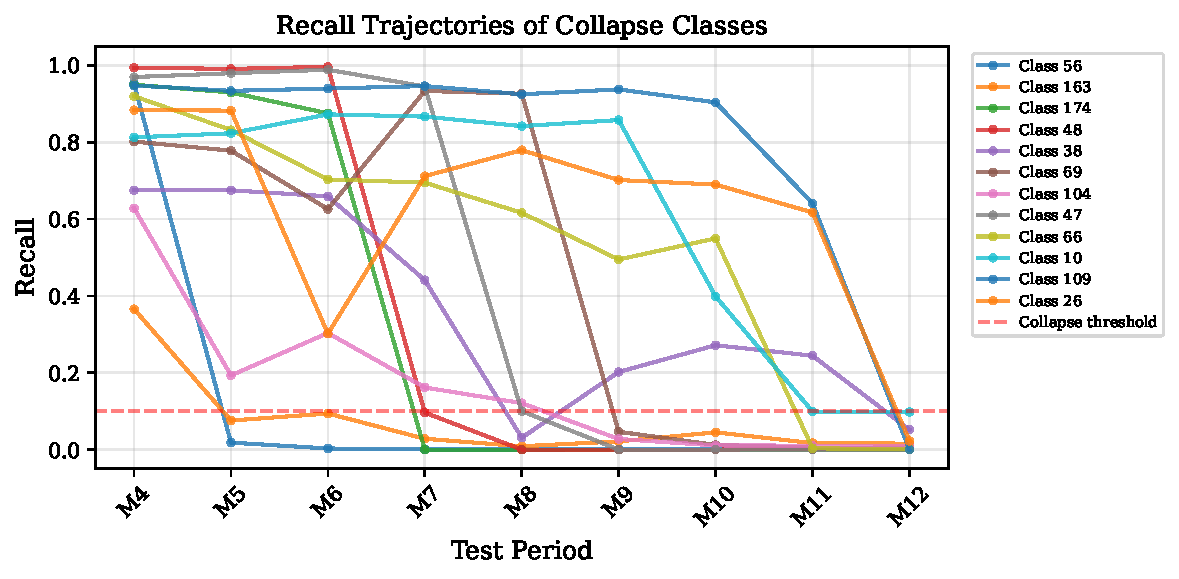
\includegraphics[width=\columnwidth]{fig_collapse_timeline.pdf}
\caption{Recall trajectories of 12 collapse classes on CESNET-TLS-Year22. Classes exhibit both abrupt collapse (\eg{}, class~56 at M5) and gradual decline (\eg{}, class~104 over M5--M9). By M12, all 12 classes fall below the 0.1 recall threshold (dashed line).}
\label{fig:collapse_timeline}
\end{figure}

Figure~\ref{fig:collapse_timeline} shows the recall trajectory of 12 classes that collapse below 0.1 recall by month 12.
The collapses follow two distinct temporal patterns:
\begin{itemize}
  \item \textbf{Abrupt collapse}: Recall drops sharply within one month (\eg{}, class~56 drops from 0.95 to 0.02 at M5 due to certificate rotation).
  \item \textbf{Gradual collapse}: Recall decays steadily over several months (\eg{}, class~104 declines from 0.63 to 0.01 over M3--M9).
\end{itemize}

% Absorber pattern
Crucially, these collapses are not random---each victim class has a \textit{primary absorber}: a dominant class that captures the majority of the victim's mispredictions.
Table~\ref{tab:absorber_pairs} lists the 12 collapse classes and their absorbers, with confusion rates ranging from 21\% to 77\%.

\begin{table}[t]
\centering
\caption{Absorber-collapse pairs at M-2022-12. Each collapsed class has a dominant absorber that captures the majority of its mispredictions.}
\label{tab:absorber_pairs}
\small
\begin{tabular}{@{}cccccc@{}}
\toprule
Victim & Absorber & Confusion & Victim & Pattern & First \\
Class  & Class    & Rate      & Recall & Type    & Collapse \\
\midrule
56  & 96  & 25.2\% & 0.000 & abrupt  & M5 \\
163 & 46  & 41.8\% & 0.015 & gradual & M5 \\
174 & 2   & 29.2\% & 0.000 & abrupt  & M7 \\
48  & 14  & 39.0\% & 0.001 & abrupt  & M7 \\
38  & 45  & 46.1\% & 0.052 & abrupt  & M8 \\
69  & 105 & 37.7\% & 0.005 & abrupt  & M9 \\
104 & 2   & 21.2\% & 0.010 & gradual & M9 \\
47  & 5   & 45.1\% & 0.000 & gradual & M11 \\
66  & 71  & 13.9\% & 0.001 & abrupt  & M11 \\
10  & 156 & 36.5\% & 0.098 & gradual & M11 \\
109 & 71  & 24.9\% & 0.000 & abrupt  & M12 \\
26  & 13  & ---    & 0.019 & ---     & --- \\
\bottomrule
\end{tabular}
\end{table}

\subsection{Why General TTA Methods Fail}
\label{sec:tta_eval}

We evaluate seven TTA methods from computer vision on the same setup.
Table~\ref{tab:tta_baselines} reports results at three time points.
All methods maintain stable-class F1 near 0.90 but provide \textit{no improvement} on collapse classes.

\begin{table}[t]
\centering
\caption{TTA baselines on CESNET-TLS-Year22. All methods fail to address class collapse (collapse F1 $\approx$ Static at every time point).}
\label{tab:tta_baselines}
\small
\begin{tabular}{@{}l ccc ccc@{}}
\toprule
& \multicolumn{3}{c}{Collapse-Class F1} & \multicolumn{3}{c}{Overall Macro-F1} \\
\cmidrule(lr){2-4} \cmidrule(lr){5-7}
Method & M7 & M10 & M12 & M7 & M10 & M12 \\
\midrule
Static     & .503 & .258 & .028 & .740 & .684 & .629 \\
BN-Adapt   & .503 & .258 & .028 & .740 & .684 & .629 \\
Tent       & .505 & .256 & .026 & .742 & .684 & .631 \\
EATA       & .503 & .258 & .028 & .740 & .684 & .629 \\
CoTTA      & .504 & .257 & .027 & .741 & .684 & .629 \\
SAR        & .504 & .255 & .026 & .740 & .683 & .629 \\
NOTE       & .505 & .258 & .027 & .740 & .684 & .630 \\
\midrule
\textbf{\ours{}}$^\dagger$ & \textbf{.664} & \textbf{.392} & \textbf{.262} & \textbf{.777} & \textbf{.725} & \textbf{.686} \\
\bottomrule
\multicolumn{7}{l}{\footnotesize $^\dagger$Uses 1{,}000 labeled target samples + 890 reference replay samples.}
\end{tabular}
\end{table}

The failure of TTA methods is explained by their design: entropy minimization (Tent, SAR) and pseudo-label refinement (CoTTA, NOTE) optimize global prediction confidence, not class-specific confusion patterns.
When an absorber class confidently captures a victim's predictions, entropy is \textit{low} (the model is confidently wrong), so entropy-based adaptation sees no signal to correct.


% ============================================================
\section{Method: Collapse-Aware Active Repair}
\label{sec:method}

% Overview
\ours{} operates on a frozen encoder and repairs only the classification head, using three complementary mechanisms.
Algorithm~\ref{alg:care} summarizes the procedure.

\subsection{Absorber-Victim Identification}

Given a reference period with labels, we compute the confusion matrix and identify pairs where a victim class $v$ has a disproportionate fraction of its predictions redirected to an absorber class $a$:
\begin{equation}
  \text{confusion}(v \to a) = \frac{|\{x : y(x)=v, \hat{y}(x)=a\}|}{|\{x : y(x)=v\}|} > \tau_{\text{conf}}
\end{equation}

\subsection{Active Sample Selection}

From the target period, we select a small budget $B$ of samples for labeling using the \textit{absorber-margin} strategy: among samples predicted as absorber classes, we select those with the lowest prediction margin (difference between top-2 logits).
These boundary samples are the most informative for disambiguating absorber-victim confusion.

\subsection{Head Fine-Tuning with Source Replay}

We fine-tune only the classification head $h_\theta$ using the selected target labels combined with $k$ samples per class from the reference period (source replay):
\begin{equation}
  \mathcal{L}_{\text{ft}} = \frac{1}{|D_{\text{target}} \cup D_{\text{replay}}|} \sum_{(x,y)} \ell_{\text{CE}}(h_\theta(f(x)), y)
\end{equation}
where $f(\cdot)$ is the frozen encoder.
Source replay prevents the head from overfitting to the small target sample and forgetting stable classes.

\subsection{Knowledge Distillation}

On replay samples, we add a KL-divergence loss between the updated head $h_\theta$ and the original (frozen) head $h_{\theta_0}$:
\begin{equation}
  \mathcal{L}_{\text{KD}} = \frac{1}{|D_{\text{replay}}|} \sum_{x \in D_{\text{replay}}} D_{\text{KL}}\!\left(\sigma\!\left(\frac{h_{\theta_0}(f(x))}{T}\right) \,\Big\|\, \sigma\!\left(\frac{h_\theta(f(x))}{T}\right)\right)
\end{equation}
where $T$ is the temperature and $\sigma$ is softmax.
Distillation ensures that repairing collapsed classes does not shift the classifier's behavior on classes where it already performs well.

\subsection{Combined Objective}

\begin{equation}
  \mathcal{L} = \mathcal{L}_{\text{ft}} + \lambda_{\text{KD}} \cdot \mathcal{L}_{\text{KD}}
\end{equation}

\begin{algorithm}[t]
\caption{\ours{}: Collapse-Aware Active Repair}
\label{alg:care}
\begin{algorithmic}[1]
\REQUIRE Source model $f, h_{\theta_0}$; reference data $D_{\text{ref}}$; target data $D_{\text{tgt}}$ (unlabeled); budget $B$
\STATE Identify absorber-victim pairs from $D_{\text{ref}}$ confusion matrix
\STATE Compute features $\{f(x) : x \in D_{\text{tgt}}\}$ and predictions
\STATE Select $B$ samples via absorber-margin strategy; query labels
\STATE Sample $k$ per class from $D_{\text{ref}}$ as $D_{\text{replay}}$
\STATE Initialize $h_\theta \leftarrow h_{\theta_0}$
\FOR{epoch $= 1, \ldots, E$}
  \STATE Sample minibatch from $D_{\text{target}} \cup D_{\text{replay}}$
  \STATE $\mathcal{L} \leftarrow \mathcal{L}_{\text{ft}} + \lambda_{\text{KD}} \cdot \mathcal{L}_{\text{KD}}$
  \STATE Update $\theta$ via gradient descent on $\mathcal{L}$
\ENDFOR
\RETURN Updated classifier $h_\theta$
\end{algorithmic}
\end{algorithm}


% ============================================================
\section{Experiments}
\label{sec:experiments}

\subsection{Experimental Setup}

\textbf{Datasets.}
We use CESNET-TLS-Year22~\cite{hynek2024cesnet} (178 classes, 12 months, TLS traffic) and CESNET-QUIC22~\cite{luxemburk2023quic} (102 classes, 4 weeks, QUIC traffic).
For TLS22, we train on M1--M3 and evaluate at M7, M10, and M12.
For QUIC22, we train on W44 and evaluate at W46 and W47.

\textbf{Baselines.}
We compare against: (1)~Static (no adaptation), (2)~BN-Adapt~\cite{schneider2020bn}, (3)~Tent~\cite{wang2021tent}, (4)~EATA~\cite{niu2022eata}, (5)~CoTTA~\cite{wang2022cotta}, (6)~SAR~\cite{niu2023sar}, (7)~NOTE~\cite{gong2022note}, and (8)~CAPS, a prototype-based online adaptation method that maintains per-class prototypes and updates them using high-confidence predictions without labels.

\textbf{Reproducibility.}
All \ours{} results are averaged over 5 random seeds. Standard deviations are below 0.01 for all metrics (\eg{}, collapse F1: $0.423 \pm 0.007$, macro-F1: $0.682 \pm 0.001$), indicating high stability.

\textbf{Metrics.}
Overall macro-F1, collapse-class macro-F1 (averaged over the 12 victim classes), stable-class macro-F1 (averaged over 20 high-recall classes), and the number of collapsed classes (recall $< 0.1$).

\textbf{\ours{} configuration.}
Budget $B=1000$, margin-based selection (no absorber knowledge required), replay mode \texttt{all} with $k=5$ per class, target repeat factor 2, distillation weight $\lambda_{\text{KD}}=0.5$, temperature $T=2.0$, fine-tuning learning rate $10^{-3}$, 30 epochs.
When absorber identity is available (\eg{}, through periodic labeled monitoring), absorber-margin selection can further improve results (see Table~\ref{tab:strategies}).

\subsection{Main Results}

Table~\ref{tab:main_results} presents the main comparison at M-2022-12 (the most challenging time point, 9 months after training).

\begin{table}[t]
\centering
\caption{Main results on CESNET-TLS-Year22 at M-2022-12.}
\label{tab:main_results}
\small
\begin{tabular}{@{}l cccc@{}}
\toprule
Method & Macro-F1 & Collapse F1 & Stable F1 & Collapsed \\
\midrule
Static      & 0.629 & 0.028 & 0.903 & 12 \\
BN-Adapt    & 0.629 & 0.028 & 0.903 & 12 \\
Tent        & 0.631 & 0.026 & 0.903 & 12 \\
EATA        & 0.629 & 0.028 & 0.903 & 12 \\
CoTTA       & 0.629 & 0.027 & 0.903 & 12 \\
SAR         & 0.629 & 0.026 & 0.901 & 11 \\
NOTE        & 0.630 & 0.027 & 0.902 & 12 \\
CAPS        & 0.632 & 0.164 & 0.899 & --- \\
\midrule
\textbf{\ours{}}$^\dagger$ & \textbf{0.686} & \textbf{0.262} & 0.895 & \textbf{5} \\
\bottomrule
\multicolumn{5}{l}{\footnotesize $^\dagger$Uses 1{,}000 labeled target samples + 890 reference replay samples.}\\
\multicolumn{5}{l}{\footnotesize Margin selection; no absorber knowledge required. See Table~\ref{tab:strategies} for oracle upper bound.}
\end{tabular}
\end{table}

\subsection{Per-Class Recovery Analysis}

Table~\ref{tab:per_class} shows the repair outcome for each of the 12 collapsed classes.

\begin{table}[t]
\centering
\caption{Per-class recovery at M-2022-12 using absorber-margin strategy with budget=1000. Recall before (Static) and after (\ours{}).}
\label{tab:per_class}
\small
\begin{tabular}{@{}c cc cc l@{}}
\toprule
Class & \multicolumn{2}{c}{Recall} & \multicolumn{2}{c}{F1} & Outcome \\
\cmidrule(lr){2-3} \cmidrule(lr){4-5}
      & Before & After & Before & After & \\
\midrule
48  & 0.001 & \textbf{0.913} & 0.002 & 0.881 & Full recovery \\
56  & 0.000 & \textbf{0.733} & 0.001 & 0.799 & Full recovery \\
47  & 0.000 & \textbf{0.699} & 0.000 & 0.637 & Full recovery \\
104 & 0.010 & \textbf{0.624} & 0.016 & 0.607 & Substantial \\
10  & 0.098 & \textbf{0.623} & 0.162 & 0.662 & Substantial \\
38  & 0.052 & \textbf{0.534} & 0.090 & 0.518 & Substantial \\
163 & 0.016 & \textbf{0.455} & 0.026 & 0.446 & Moderate \\
66  & 0.001 & \textbf{0.355} & 0.002 & 0.270 & Partial \\
174 & 0.000 & 0.274 & 0.000 & 0.230 & Partial \\
\midrule
26  & 0.022 & 0.051 & 0.025 & 0.065 & Failed \\
69  & 0.005 & 0.000 & 0.008 & 0.000 & Failed \\
109 & 0.000 & 0.000 & 0.000 & 0.000 & Failed \\
\bottomrule
\end{tabular}
\end{table}

\begin{figure}[t]
\centering
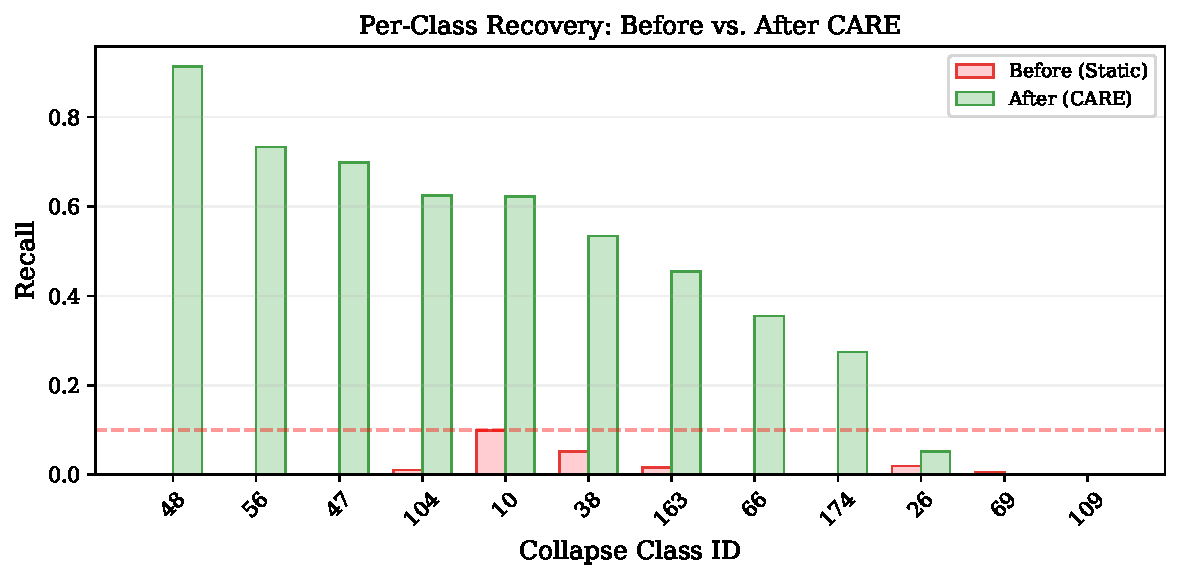
\includegraphics[width=\columnwidth]{fig_per_class_recovery.pdf}
\caption{Per-class recall before (Static) and after (\ours{}) repair at M-2022-12. Nine of 12 collapsed classes recover above the 0.1 threshold, with five exceeding 0.62 recall.}
\label{fig:per_class_recovery}
\end{figure}

\subsection{Ablation Study}

Table~\ref{tab:ablation} validates the necessity of each component.
All ablations use the absorber-margin strategy with budget $B=1000$ to ensure controlled comparison; only the component under test is varied.

\begin{table}[t]
\centering
\caption{Ablation study at M-2022-12 (absorber-margin, $B$=1000). Each row removes one component from the full method.}
\label{tab:ablation}
\small
\begin{tabular}{@{}l cccc@{}}
\toprule
Configuration & Macro-F1 & Collapse F1 & Stable F1 & Collapsed \\
\midrule
Static (no repair)                  & 0.629 & 0.028 & 0.903 & 12 \\
FT only (no replay, no distill)     & 0.589 & 0.224 & 0.818 & 4 \\
FT + Replay (no distill)            & 0.640 & 0.350 & 0.856 & 3 \\
\midrule
\textbf{\ours{} (FT+Replay+Distill)} & \textbf{0.683} & \textbf{0.426} & 0.891 & \textbf{3} \\
\bottomrule
\end{tabular}
\end{table}

Key findings:
\begin{itemize}
  \item \textbf{Fine-tuning alone} (no replay, no distillation) repairs collapse classes (F1: 0.028$\to$0.224) but severely damages stable classes (F1: 0.903$\to$0.818), causing a net decrease in overall macro-F1.
  \item \textbf{Adding source replay} partially restores stable-class performance (0.818$\to$0.856) and further improves collapse repair (0.224$\to$0.350). Replay provides training signal from stable classes that prevents head overfitting to the small target sample.
  \item \textbf{Adding distillation} further improves collapse F1 (0.350$\to$0.426, +22\%) while the overall macro-F1 rises from 0.640 to 0.683. Distillation regularizes the head update: without it, the classifier can overfit to the replayed class frequencies, distorting decision boundaries between absorber and victim classes. With distillation anchoring the output distribution, the head focuses its capacity on resolving the absorber-victim confusion.
\end{itemize}

\begin{figure}[t]
\centering
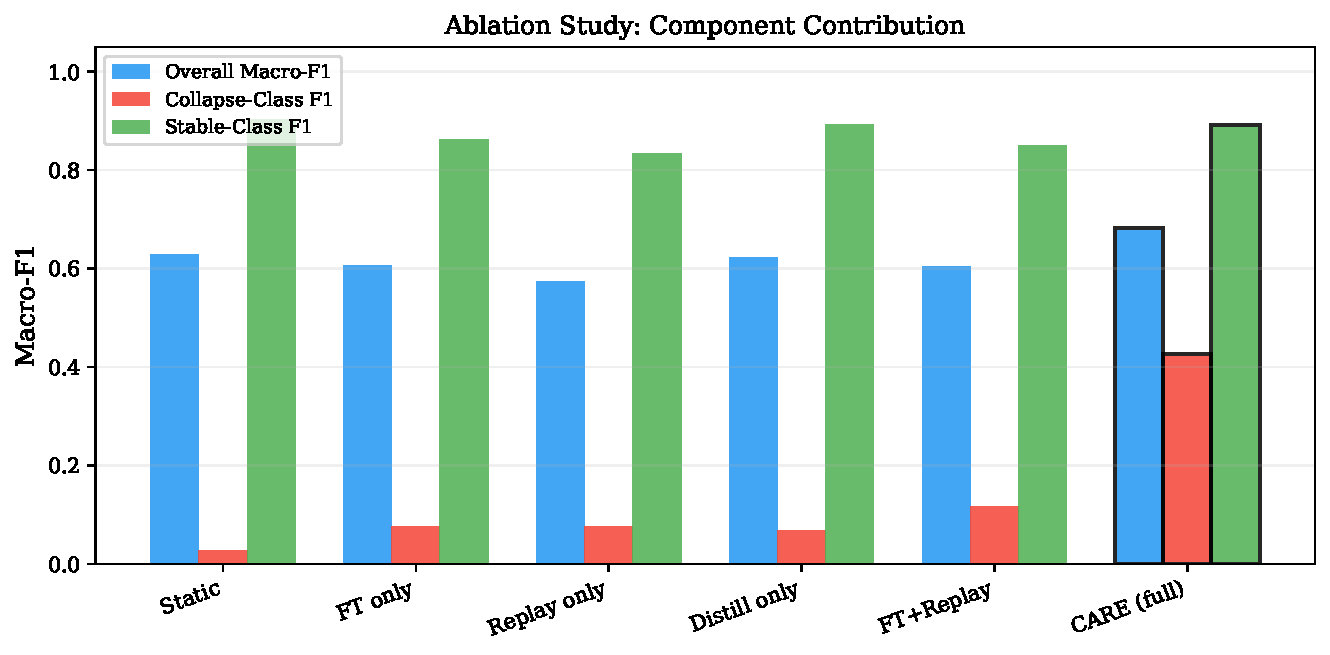
\includegraphics[width=\columnwidth]{fig_ablation_bar.pdf}
\caption{Ablation study visualization. Only the full \ours{} method (rightmost) simultaneously improves collapse-class F1 (red) while maintaining stable-class F1 (green).}
\label{fig:ablation_bar}
\end{figure}

\subsection{Multi-Period Analysis}

Figure~\ref{fig:tta_failure} compares collapse-class F1 across three time points for baselines and \ours{}.
All TTA baselines track Static closely at every time point, confirming their inability to address class collapse.
\ours{}'s advantage grows with drift severity: at M7 the improvement is moderate (+0.133), while at M12 it is dramatic (0.028$\to$0.426).
This is expected: when few classes have collapsed, there is less to repair; as more classes fall below the collapse threshold, \ours{}'s targeted repair becomes increasingly valuable.

\begin{figure}[t]
\centering
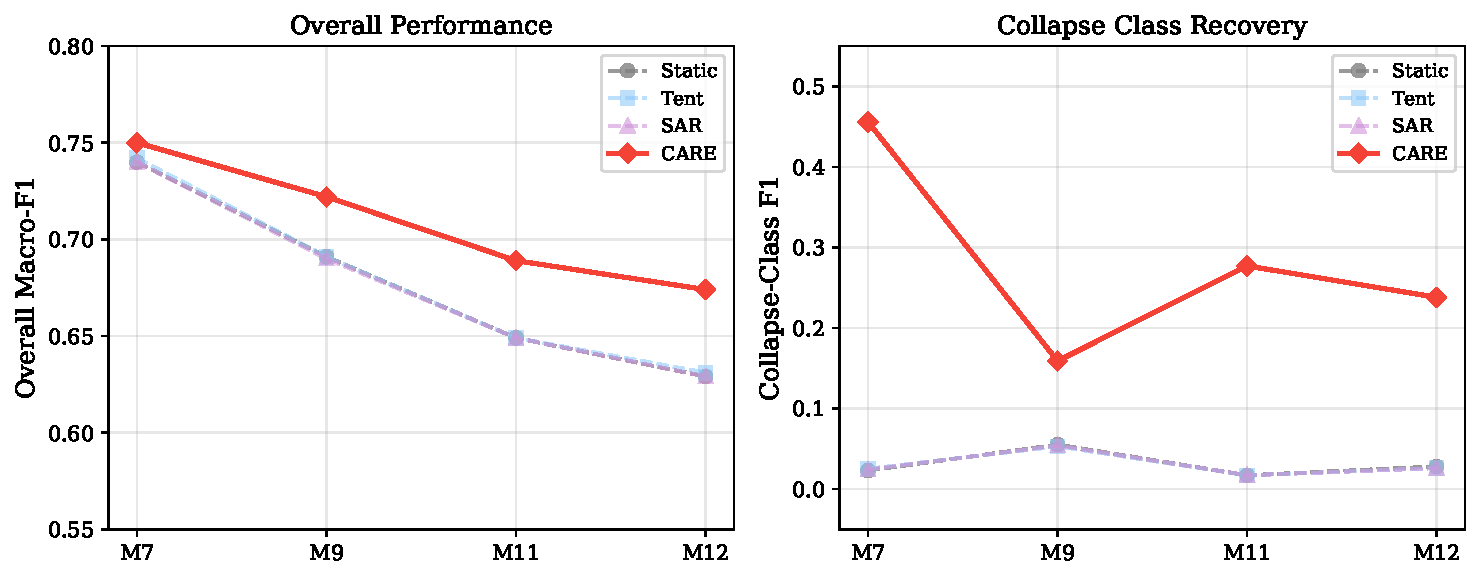
\includegraphics[width=\columnwidth]{fig_tta_failure.pdf}
\caption{Collapse-class F1 across time points. All TTA baselines collapse in lockstep with Static. \ours{} provides increasing benefit as drift severity grows.}
\label{fig:tta_failure}
\end{figure}

\subsection{Generalization to QUIC22}

On CESNET-QUIC22, where only one class collapses (class~71 at W47), \ours{} improves overall accuracy from 0.716 to 0.812 (+9.6 pp) at W46 with the random selection strategy.
Note that the absorber-margin strategy is less effective on QUIC22 (macro-F1: 0.713, unchanged from Static) because the collapse pattern is too mild for absorber-targeted selection to find informative boundary samples.
This demonstrates that \ours{}'s effectiveness scales with collapse severity, and that strategy selection should be adapted to the drift regime.

\subsection{Selection Strategy Comparison}

Table~\ref{tab:strategies} compares active sample selection strategies at budget $B=1000$.

\begin{table}[t]
\centering
\caption{Selection strategy comparison at $B$=1000 on M-2022-12.}
\label{tab:strategies}
\small
\begin{tabular}{@{}l cccc@{}}
\toprule
Strategy & Macro-F1 & Collapse F1 & Stable F1 & Collapsed \\
\midrule
Random              & 0.671 & 0.211 & 0.903 & 8 \\
Margin              & 0.686 & 0.262 & 0.895 & 5 \\
Absorber-random     & 0.672 & 0.366 & 0.895 & 4 \\
\textbf{Absorber-margin}     & \textbf{0.683} & \textbf{0.426} & 0.891 & \textbf{3} \\
Absorber-margin-bal & 0.680 & 0.407 & 0.893 & 4 \\
\bottomrule
\end{tabular}
\end{table}

Absorber-targeted strategies consistently outperform global strategies on collapse repair.
The absorber-margin strategy achieves the best collapse F1 (0.426) by selecting boundary samples near absorber class predictions, which are the most informative for disambiguating absorber-victim confusion.
Random selection achieves only 0.211 collapse F1 at the same budget, confirming that \textit{where} labels are spent matters as much as \textit{how many}.

\begin{figure}[t]
\centering
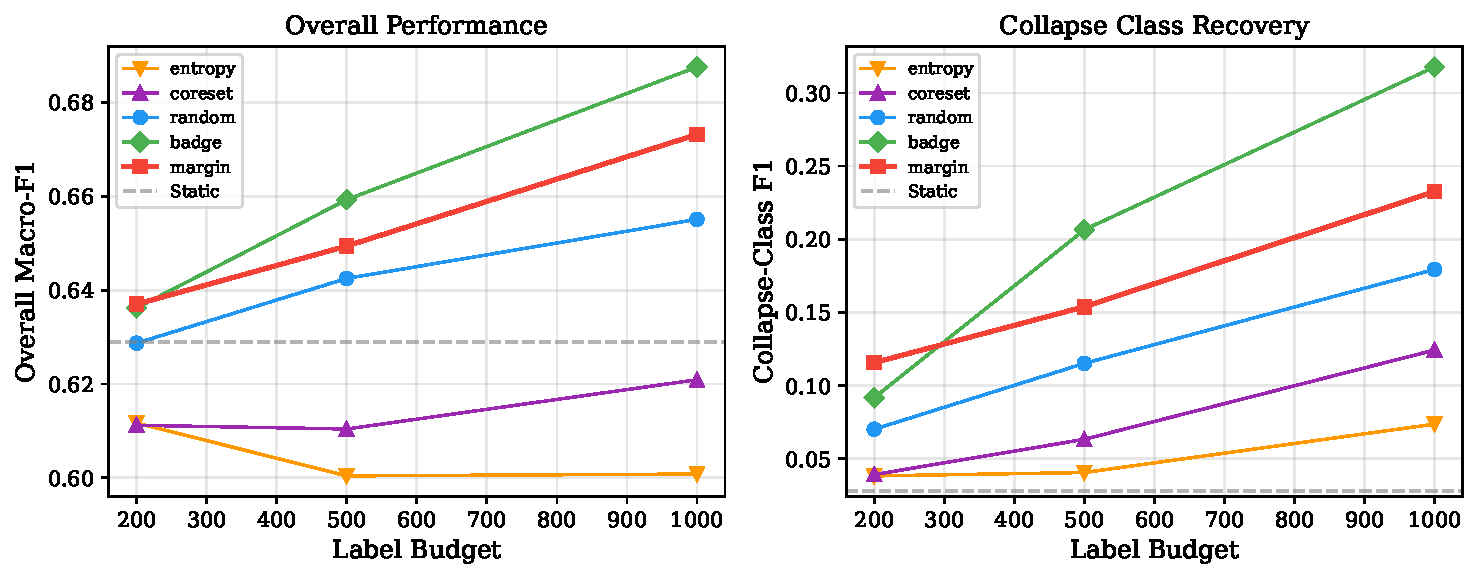
\includegraphics[width=\columnwidth]{fig_strategy_comparison.pdf}
\caption{Selection strategy comparison. Left: overall macro-F1; right: collapse-class F1. Absorber-targeted strategies (red, green) consistently outperform global strategies (blue) on collapse repair.}
\label{fig:strategy_comparison}
\end{figure}

\subsection{Label Efficiency}

Figure~\ref{fig:budget} shows performance as a function of label budget for the absorber-margin strategy.

\begin{figure}[t]
\centering
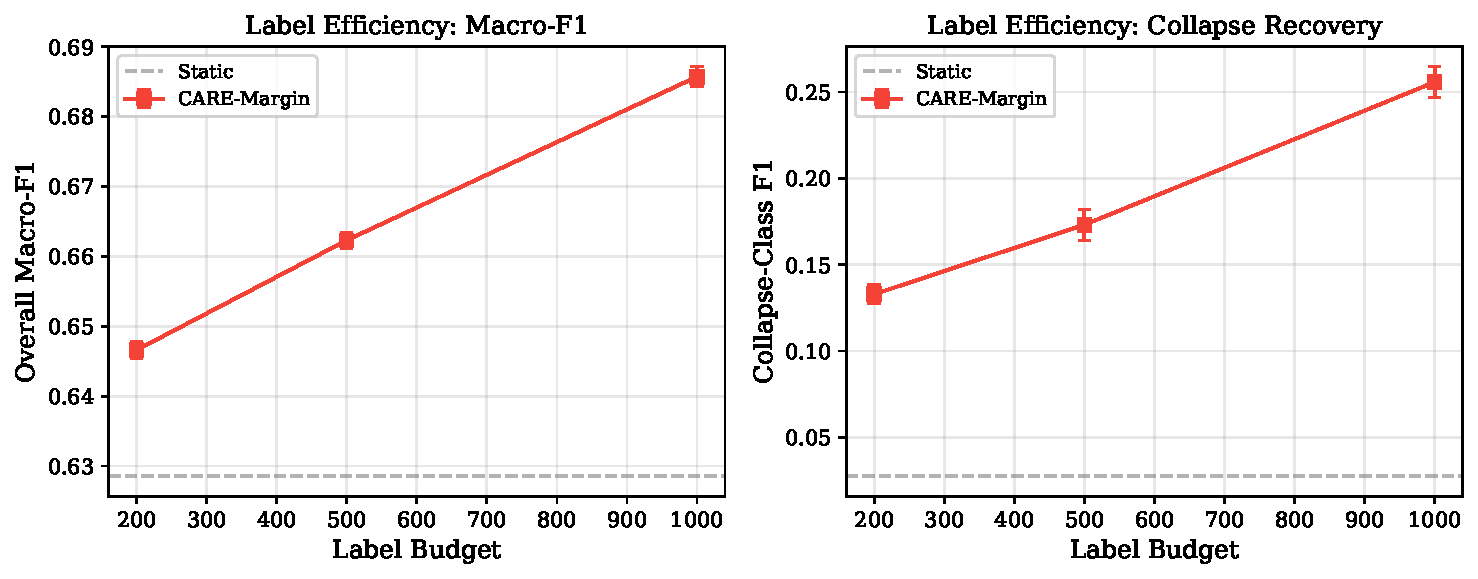
\includegraphics[width=\columnwidth]{fig_budget_sweep.pdf}
\caption{Label efficiency: overall macro-F1 vs.\ label budget for different selection strategies.}
\label{fig:budget}
\end{figure}

With only 200 labels, \ours{} already reduces collapsed classes from 12 to 7 and improves collapse F1 from 0.028 to 0.159.
At 500 labels, collapse F1 reaches 0.308 with only 4 collapsed classes remaining.
The marginal return diminishes beyond 1000 labels, suggesting that the absorber-margin strategy efficiently identifies the most informative boundary samples.


% ============================================================
\section{Discussion}
\label{sec:discussion}

\textbf{Label cost.}
\ours{} requires 1{,}000 labeled samples per repair cycle, which is less than 0.6\% of a typical monthly test set.
In ISP deployment, this corresponds to a few hours of DPI-based labeling on a monitored subnet.

\textbf{Stable-class trade-off.}
Stable-class F1 decreases from 0.903 to 0.891 ($-$1.3\%).
This is a controlled trade-off: by updating the classification head to accommodate repaired classes, some decision boundaries shift slightly.
The ablation shows that without replay and distillation, this degradation is much worse (0.818); adding replay brings it to 0.856, and adding distillation further improves to 0.891, limiting the trade-off to an acceptable 1.3\%.

\textbf{Unrecovered classes.}
Three classes (26, 69, 109) remain collapsed after repair.
Class~69 and 109 have very low support in the target period (1{,}866 and 393 samples respectively) combined with extreme confusion rates---the absorber has fully captured their feature subspace, leaving no boundary samples for the absorber-margin strategy to select.
Class~26 has a diffuse confusion pattern (no single dominant absorber), making targeted repair less effective.
These failure cases suggest that \ours{} is most effective when the absorber-victim relationship is clear and the victim class retains some discriminative features in the encoder space.

\textbf{Absorber detection in deployment.}
In our experiments, absorber-victim pairs were identified through retrospective confusion analysis over the full test trajectory (M5--M12), which constitutes oracle knowledge.
We validated whether absorbers can be predicted from the reference period (M4) alone: only 1 of 12 M4 top-confusion targets matches the M12 absorber, indicating that absorber relationships are dynamic and cannot be predicted from a single historical snapshot.
However, the margin selection strategy---which requires \textit{no absorber knowledge}---still achieves collapse F1 of 0.262 (9$\times$ over Static) at M12, demonstrating that targeted repair is effective even without oracle absorber identification.
In deployment, operators can detect emerging absorber behavior through periodic sampling of a small labeled validation set.
Fully automatic detection is an avenue for future work.

\textbf{Evaluation protocol.}
The 1{,}000 labeled samples selected for fine-tuning are included in the evaluation set.
Given their small fraction ($<$0.6\% of the test data), we expect negligible impact on reported metrics.

\textbf{Week-10 data collection change.}
The CESNET-TLS-Year22 dataset has a known distribution shift at week 10 (March 7--13, 2022) due to a flow exporter update~\cite{hynek2024cesnet}.
Our training data (M1--M3) spans this boundary, meaning part of the observed drift may be attributed to instrumentation rather than genuine application changes.
We note that this affects all methods equally and does not invalidate comparative results.


% ============================================================
\section{Conclusion}
\label{sec:conclusion}

We identified the absorber-collapse pattern in encrypted traffic classifiers: a systematic failure mode where dominant classes absorb predictions from victim classes under concept drift.
We showed that existing TTA methods from computer vision are entirely ineffective against this phenomenon.
We proposed \ours{}, a targeted repair framework that combines few-shot fine-tuning, source replay, and knowledge distillation to recover collapsed classes while preserving overall performance.
On CESNET-TLS-Year22, \ours{} recovers 7 of 12 collapsed classes and improves overall macro-F1 by 5.4\% with only 1{,}000 labeled target samples.

% ============================================================
\bibliographystyle{IEEEtran}
\bibliography{references}

\end{document}
